\section{Redes Neurais}

\abbrev{RNN}{redes neurais recorrentes}
\subsubsection{RNN}
Redes neurais recorrentes (RNNs, do inglês \textit{recurrent neural networks})
 são apropriadas para dados que tenham uma relação de sequência entre si
 \cite{gru4rec_1}. Sua principal diferença em relação aos demais modelos de
 aprendizado profundo é a existência de um estado oculto $\mathbf{h_t}$ em
 cada unidade da rede, cujo valor é obtido a partir da seguinte função de
 atualização:
 \symbl{$\mathbf{h_t}$}{estado oculto da unidade no instante $t$}
\begin{equation}
    \mathbf{h_t} = g(W\mathbf{x_t} + U\mathbf{h_{t-1}})
\end{equation}
onde $g$ é uma função suave e limitada entre 0 e 1, como uma função logística
sigmoide ou tangente hiperbólica, $\mathbf{x_t}$ é a entrada da unidade no
instante atual, $W$ e $U$ são os pesos associados à entrada e ao estado
anterior, $\mathbf{h_{t-1}}$ é o estado no instante anterior. Uma RNN gera uma
distribuição de probabilidade sobre o próximo elemento da sequência a partir do
estado atual:

\begin{equation}
    p(\mathbf{x_t}|\mathbf{x_1},\ldots , \mathbf{x_{t-1}}) = g(\mathbf{h_t})
\end{equation}

Um problema típico da arquitetura básica de RNNs é o desaparecimento ou explosão
do gradiente ao minimizar a função de custo, uma vez que o incremento ou
decremento do gradiente equivale ao produtório dos pesos de todas as unidades, o
que converge para um valor minúsculo ou diverge para um valor enorme. Unidades
sob a forma de LSTMs ou GRUs foram propostas para resolver esse problema.


\subsubsection{LSTM}
\abbrev{LSTM}{memória de curto e longo prazo}
A memória de curto e longo prazo (LSTM, do inglês \textit{long short-term
memory}) \cite{chung2014empirical} substitui a unidade típica de uma RNN. Sua
principal melhoria, tanto na LSTM é a capacidade de manter o estado atual
de suas células, em vez de sobrescrevê-lo a cada iteração. Dessa forma, a
unidade pode detectar e manter informações relevantes de forma dinâmica,
inclusive em sequências longas.

Sua arquitetura resolve os problemas de dissipação ou explosão do
gradiente, uma vez que a etapa de \textit{backpropagation} não envolve a
multiplicação de todos os pesos.

A LSTM é composta por uma célula de memória $\mathbf{c_t}$. A saída, ou ativação
$\mathbf{h_t}$, é dada por:
\begin{equation}
    \mathbf{h_t} = \mathbf{o_t}\tanh(\mathbf{c_t})
\end{equation}
em que $\mathbf{o_t}$ é a porta de saída, a qual controla a quantidade de
exposição, cujo valor é dado por:

\begin{equation}
    \mathbf{o_t} = \sigma(W_o\mathbf{x_t} + U_o\mathbf{h_{t-1}} + V_o\mathbf{c_t})
\end{equation}
em que $\sigma$ é a função logística sigmoide, $W_o$, $U_o$ e $V_o$ são as
matrizes de pesos.
\symbl{$\sigma(\cdot)$}{função logística sigmoide}

A memória da célula $\mathbf{c_t}$ é atualizada a partir da memória anterior
$\mathbf{c_{t-1}}$ e do estado candidato $\mathbf{\tilde{c}_t}$, ambos ponderados
respectivamente pelas portas de esquecimento $\mathbf{f_t}$ e de entrada $\mathbf{i_t}$:
\begin{align}
    \mathbf{c_t} &= \mathbf{f_t} \odot \mathbf{c_{t-1}} + \mathbf{i_t} \odot \mathbf{\tilde{c}_t} \\
    \mathbf{f_t} &= \sigma(W_f\mathbf{x_t} + U_f\mathbf{h_{t-1}} + V_f\mathbf{c_{t-1}}) \\
    \mathbf{i_t} &= \sigma(W_i\mathbf{x_t} + U_i\mathbf{h_{t-1}} + V_i\mathbf{c_{t-1}})
\end{align}
sendo o operador $\odot$ o produto
de Hadamard. O novo estado da célula é dado por:
\symbl{$\odot$}{operador produto de Hadamard}

\begin{equation}
    \mathbf{\tilde{c}_t} = \tanh(W_c\mathbf{x_t} + U_c\mathbf{h_{t-1}})
\end{equation}


\subsubsection{GRU}
\abbrev{GRU}{unidade recorrente fechada}
Assim como a LSTM, a unidade recorrente fechada (GRU, do inglês \textit{gated
recurrent unit}), também possui estados auxiliares, denominados portas, que
controlam a atualização de seu estado principal, e ambas realizam a soma linear
entre o estado anterior com o estado candidato. A principal diferença entre
essas duas unidades é a capacidade da LSTM controlar o quanto do estado anterior
é assimilado, o que não há na GRU.

Na GRU, porta de atualização $\mathbf{z_t}$ pondera o quanto do
estado candidato $\mathbf{\hat{h_t}}$ e do estado anterior $\mathbf{h_{t-1}}$
são mantidos ou descartados:
\begin{equation}
    \mathbf{h_t} = (1 - \mathbf{z_t})\mathbf{h_{t-1}} + \mathbf{z_t}\mathbf{\hat{h}_t}
\end{equation}
onde a porta de atualização $\mathbf{z_t}$, o estado candidato $\mathbf{\hat{h_t}}$
e a porta de reinício $\mathbf{r_t}$ são dadas pelas equações:
\begin{align}
    \mathbf{z_t} &= \sigma(W_z\mathbf{x_t} + U_z\mathbf{h_{t-1}}) \\
    \mathbf{\hat{h}_t} &= \tanh(W_x\mathbf{x_t} + U_r(\mathbf{r_t} \odot \mathbf{h_{t-1}})) \\
    \mathbf{r_t} &= \sigma(W_r\mathbf{x_t} + U_r\mathbf{h_{t-1}})
\end{align}
em que $\sigma$ é a função logística sigmoide.

\subsubsection{Codificador-Decodificador}
Uma arquitetura típica de redes neurais utiliza um par codificador-decodificador
em tarefas que recebem uma sequência de palavras, símbolos, dados ou sessões na
entrada, retornando a sequência mais provável na saída
\cite{bahdanau2016neural}. Por exemplo, em tarefas de tradução, o codificador e
o decodificador são treinados conjuntamente para maximizar a probabilidade de
uma tradução correta, dada uma frase inserida na entrada do modelo.

\vspace{1cm}
\begin{figure}[htbp]
    \centering
    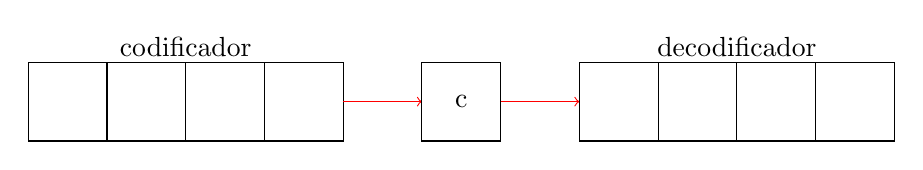
\begin{tikzpicture}
        % Draw rectangles
        \draw (0,0) rectangle (1,1); % First square
        \draw (1,0) rectangle (2,1); % Second square
        \draw (2,0) rectangle (3,1); % Third square
        \draw (3,0) rectangle (4,1); % Fourth square
      
        % Add text "encoder" above the rectangle
        \node at (2,1.2) {codificador};
        
        % Draw error line
        \draw[->, red] (4,0.5) -- (5,0.5); % Error line
        
        % Draw horizontal rectangle named "c"
        \draw (5,0) rectangle (6,1); % Rectangle "c"
        \node at (5.5,0.5) {c}; % Text "c" inside rectangle
        
        % Draw arrow to decoder
        \draw[->, red] (6,0.5) -- (7,0.5); % Arrow to decoder
        
        % Draw rectangles for decoder
        \draw (7,0) rectangle (8,1); % First square
        \draw (8,0) rectangle (9,1); % Second square
        \draw (9,0) rectangle (10,1); % Third square
        \draw (10,0) rectangle (11,1); % Fourth square
        % Add text "decoder" above the rectangle
        \node at (9,1.2) {decodificador};
      \end{tikzpicture}
      \caption{Encoder-Decoder Framework}

\end{figure}

Nessa arquitetura, o codificador lê um vetor de entrada $\mathbf{x}$ e retorna
um vetor intermediário $\mathbf{c}$, tal que:   
\begin{align}
    \mathbf{h_t} &= f(\mathbf{x_t}, \mathbf{h_{t-1}}) \\
    \mathbf{c} &= q(\mathbf{h_1}, \ldots, \mathbf{h_{T_x}})
\end{align}
em que $h_t \in \mathbb{R}^n$ é o estado oculto no instante $t$, $\mathbf{c}$ é o vetor
gerado a partir da sequência dos estados ocultos, $f$ é uma função não-linear,
como uma unidade LSTM, e $q(\cdot)$ é uma função sobre os estados ocultos. Por
exemplo, caso a função $q$ retorne apenas o último estado, $q(\cdot) =
\mathbf{h_{T_x}}$.

O decodificador é treinado para prever a próxima palavra $\mathbf{y_t}$, dado o
vetor intermediário $\mathbf{c}$ e todas as palavras previamente preditas
$\mathbf{y_1}, \ldots, \mathbf{y_{t-1}}$. O decodificador define uma
distribuição de probabilidade conjunta sobre a tradução $\mathbf{y}$, decompondo
a probabilidade conjunta em probabilidades condicionais ordenadas:
\begin{equation}
    p(\mathbf{y}) = \prod_{t=1}^T p(y_t | y_1, \ldots, y_{t-1}, \mathbf{c})
\end{equation}
\begin{equation}
    p(y_t | y_1, \ldots, y_{t-1}, \mathbf{c}) = g(y_{t-1}, \mathbf{s_t}, \mathbf{c})
\end{equation}
em que $g$ é uma função não-linear que retorna a probabilidade de
$\mathbf{y_t}$, sendo $\mathbf{s_t}$ o estado oculto de $y_t$ na saída.

Um problema dessa arquitetura é a menor qualidade de informação transmitida pelo
vetor intermediário na saída do codificador, que comprime a frase na entrada a
partir dos estados ocultos. Essa característica faz com que a taxa de acerto do
modelo diminua conforme o comprimento da frase de entrada aumenta. Essa
deterioração da taxa de acerto é resolvida ao incluir o mecanismo de atenção
na arquitetura.

\subsubsection{Mecanismo de atenção}
Modelos sequenciais ou recorrentes, durante o processo de treinamento, efetuam
uma série de cálculos de forma sequencial, uma vez que cada estado oculto
$\mathbf{h_t}$ depende do estado anterior $\mathbf{h_{t-1}}$ e da entrada no
estado atual $\mathbf{x_t}$. Esse processo sequencial impede a paralelização, o
que gera um gargalo de processamento.

O mecanismo de atenção \cite{bahdanau2016neural} resolve esse problema ao
receber conjuntamente todos os estados ocultos, cuja importância de cada um é
ponderada pelos pesos de atenção $\mathbf{\alpha_{ij}}$:


\begin{align}
    c_i &= \sum_{j=1}^{T_x} \alpha_{ij} \mathbf{h_j} \\
    \alpha_{ij} &= \frac{\exp(e_{ij})}{\sum_{k=1}^{T_x} \exp(e_{ik})} \\
    \alpha_{ij} &=  \text{softmax}(e_{ij})
\end{align}

Cada peso de atenção é obtido a partir de um modelo de alinhamento $\mathbf{e}$,
que identifica a relevância conjunta das entradas em torno da posição $i$ e das
saídas em torno da posição $j$ entre si. O ato de atribuir pesos de atenção a
cada estado oculto é denominado \textit{pooling} de atenção.

O modelo de alinhamento é uma camada de
rede neural, obtida por:

\begin{equation}
    e_{ij} = a(\mathbf{s_{i-1}}, \mathbf{h_j}) = \mathbf{v_a}^\top \tanh(\mathbf{W_a}s_{i-1} + \mathbf{U_a}h_j)
\end{equation}
em que $\mathbf{v_a} \in \mathbb{R}^n$, $\mathbf{W_a} \in \mathbb{R}^{n \times
n}$ e $\mathbf{U_a} \in \mathbb{R}^{n \times m}$ são as matrizes com os pesos da
camada.

\subsubsection{Auto-atenção}
Auto-atenção (do inglês \textit{self-attention}) é uma forma de mecanismo de
atenção cujos pesos dependem apenas de uma única sequência, em vez de duas
sequências distintas \cite{kim2017structured}. O mecanismo de atenção
tradicional não modela diretamente as dependências entre os elementos da
sequência de entrada, mas sim a relação entre os estados ocultos do codificador
e do decodificador. O uso mais reconhecido do mecanismo de auto-atenção ocorre
na arquitetura de transformadores (do inglês \textit{transformers}), que
viabilizam o uso do mecanismo de atenção em modelos que não sejam
necessariamente sequenciais, como as redes neurais recorrentes.

A arquitetura de transformadores replica a estrutura do mecanismo de
auto-atenção em diferentes locais de sua arquitetura. Essa estrutura calcula a
atenção a partir de três matrizes de pesos: consultas (do inglês
\textit{queries}), chaves (do inglês \textit{keys}) e valores (do inglês
\textit{values}), dadas respectivamente pelas matrizes $\mathbf{Q}$,
$\mathbf{K}$ e $\mathbf{V}$. $\mathbf{Q}$ e $\mathbf{K}$ são matrizes de dimensões $d_k
\times n$ e $\mathbf{V}$ de dimensões $d_v \times n$, em que $d_k$ e $d_v$
são as dimensões dos \textit{embeddings}.


As matrizes Q, K e V modelam, respectivamente, a
relevância do \textit{embedding} de entrada, a relevância do \textit{embedding}
de saída e a probabilidade dos elementos do \textit{embedding} de saída.
Dessa forma, a atenção é calculada a partir da similaridade entre as matrizes de
consultas e chaves, ponderada pela matriz de valores:

\begin{equation}
    \text{Attention}(\mathbf{Q}, \mathbf{K}, \mathbf{V}) = \text{softmax}(\frac{\mathbf{QK}^\top}{\sqrt{d_k}})\mathbf{V}
\end{equation}
em que $\sqrt{d_k}$ é o fator de escala, que normaliza o produto escalar entre
as matrizes de consultas e chaves.

\subsubsection{CNN}
\abbrev{CNN}{redes neurais convolucionais}
Redes neurais convolucionais (CNNs, do inglês \textit{convolutional neural
networks}), criadas para tarefas de síntese e análise de imagens, incluindo
classificação, detecção, segmentação, restauração de imagens, entre outras.
Também são aplicadas em tarefas de análise de dados sequencias ou com alguma
estrutura espacial \cite{Bishop:DeepLearning24}. As CNNs foram as primeiras
redes neurais profundas a serem implementadas e distribuídas com sucesso em
aplicações práticas \cite{lecun1989}.

A primeira camada da CNN atribui um peso a cada região da imagem. Essa região é
o campo receptivo de uma unidade, cujas características são analisadas.
Os pesos formam um filtro em formato de matriz bi-dimensional, denominado
núcleo. A combinação linear do núcleo com a intensidade dos píxeis da imagem é
aplicada a uma função não-linear, detectando a presença ou ausência da
característica que aquele núcleo em particular é responsável por detectar:

\symbl{$\text{ReLU}(\cdot)$}{unidade linear retificada}
\begin{equation}
    z = \text{ReLU}(\mathbf{w}^\text{T} \mathbf{x} + w_0)
\end{equation}

Ao aplicar o mesmo núcleo em diferentes regiões da imagem, obtém-se um mapa de
ativação, que é uma representação da imagem com as características detectadas
pelo núcleo. Esse procedimento é realizado pela operação de convolução.

A partir de uma imagem $\mathbf{I}$ com píxeis de intensidade $I(j, k)$
e do filtro $\mathbf{K}$ com valores $K(l, m)$, gera-se um mapa $\mathbf{C}$ com
os valores de ativação dados por:

\begin{equation}
    C(j, k) = \sum_{l} \sum_{m} I(j+l, k+m)K(l, m)
\end{equation}
a operação acima, na bibliografia de aprendizado de máquina, é denominada
convolução, representada por $\mathbf{C} = \mathbf{I} * \mathbf{K}$. O mapa de
ativação da camada oculta é obtido ao calcular a função de ativação para cada
unidade. De forma mais rigorosa, a operação citada é uma correlação cruzada, dado
que a convolução e a convolução circular no contexto de processamento de sinais
satisfazem uma série de propriedades que não cabem à correlação cruzada.

Algumas operações auxiliares são utilizadas: o \textit{padding}, que consiste em
preencher com zeros o mapa de ativações, de forma a manter a dimensão da imagem
original; o \textit{stride}, que consiste em deslocar o filtro de forma a
aumentar a distância entre as regiões da imagem que serão analisadas; e o
\textit{pooling}, que consiste em reduzir a dimensionalidade do mapa de
ativações, mantendo apenas os valores mais relevantes. Além disso, imagens
coloridas são representadas por três matrizes, uma para cada canal de cor. Dessa
forma, a representação da imagem e das camadas ocultas são realizadas por
tensores.

Para implementar a rede convolucional em múltiplas camadas, cada camada é
seguida das operações de \textit{pooling} e convolução, reduzindo a
dimensionalidade. Em geral, as últimas camadas são compostas por camadas
totalmente conectadas com uma função de ativação na saída, analisando de forma
mais completa a relação entre as características detectadas pelas camadas.

\subsubsection{GNN}
\abbrev{GNN}{redes neurais de grafos}
A representação em grafos torna possível identificar padrões
não-triviais entre os dados. Também são facilmente interpretáveis, o que
permite a aplicação de uma variedade de métodos de aprendizado de máquina. Um
desses métodos é o aprendizado profundo em redes neurais de grafos (GNNs, do
inglês \textit{graph neural networks}).


Na notação formal, o grafo $\mathcal{G} = (\mathcal{V}, \mathcal{E})$ consiste no conjunto de
vértices ou nós $\mathcal{V}$ e arestas $\mathcal{E}$. A aresta que conecta
o nó $n$ ao nó $m$ é denotada pela tupla $(n, m)$. Dois nós são adjacentes ou vizinhos
se estiverem conectados por uma aresta, tal que o conjunto dos nós adjacentes a $n$
é dado por $\mathcal{N}(n) = \{m : (n, m) \in \mathcal{E}\}$.
\symbl{$\mathcal{G}$}{grafo}
\symbl{$\mathcal{V}$}{conjunto de vértices de um grafo}
\symbl{$\mathcal{E}$}{conjunto de arestas de um grafo}
\symbl{$\mathcal{N}(n)$}{conjunto de nós adjacentes ao nó $n$ em um grafo}

A estrutura básica de uma GNN é composta por nós que recebem e agregam
informações de sua vizinhança a cada iteração. Os nós vizinhos também agregam
informações de seus nós adjacentes e assim por diante, formando uma estrutura de
árvore, convergindo para um determinado nó. Essa estrutura é representada
igualmente em uma sequência de camadas, tal que cada camada equivale ao passo de
iteração seguinte ao da camada anterior.

Para o n-ésimo nó e a l-ésima camada da rede, obtém-se o vetor-coluna
$\mathbf{h}^{(l)}_n$ contendo o \textit{embedding} do nó, em que
$\mathbf{h}^{0}_n = \mathbf{x}_n$. O vetor $\mathbf{z}^{l}_n$ é responsável
por agregar as informações transmitidas pelos nós vizinhos. Dados os operadores
de agregação e atualização, que são funções diferenciáveis, temos que \cite{Bishop:DeepLearning24}:

\begin{align}
    \mathbf{z}^{(l)}_n &= \text{AGREGA}( \{ \mathbf{h}^{(l)}_m : \forall m \in \mathcal{N}(n)\} ) \label{eq:agrega} \\
    \mathbf{h}^{(l+1)}_n &= \text{ATUALIZA}(\mathbf{h}^{(l)}_n, \mathbf{z}^{(l)}_n) \label{eq:atualiza}
\end{align}
sendo a saída da rede neural igual a $\{h^{L}_n\}$, que é o conjunto dos
\textit{embeddings} dos nós na última camada $L$, tal que $l \in {0, \ldots,
L}$. A figura \ref{fig:gnn}, adaptada de \citet{graph_rep_learning}, ilustra
a vizinhança do nó amarelo enquanto estado $\mathbf{h}^{(l+1)}_n$.

\vspace{2em}
\begin{figure}[ht]
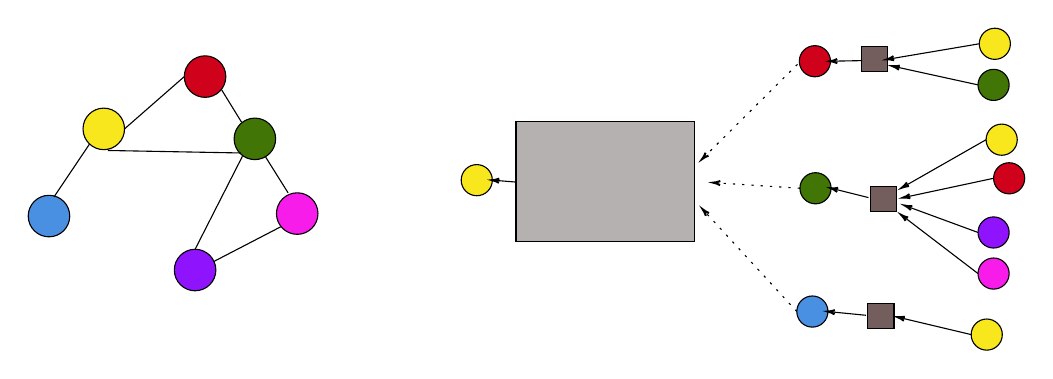
\begin{tikzpicture}[x=0.75pt,y=0.75pt,yscale=-1,xscale=1]
\tikzset{every picture/.style={line width=0.75pt}} %set default line width to 0.75pt        
\begin{scope}[scale=0.4, transform shape, shift={(0,50)}]
%Shape: Circle [id:dp7391127131517923] 
\draw  [fill={rgb, 255:red, 248; green, 231; blue, 28 }  ,fill opacity=1 ] (149,102) .. controls (149,88.19) and (160.19,77) .. (174,77) .. controls (187.81,77) and (199,88.19) .. (199,102) .. controls (199,115.81) and (187.81,127) .. (174,127) .. controls (160.19,127) and (149,115.81) .. (149,102) -- cycle ;
%Shape: Circle [id:dp5040331320120275] 
\draw  [fill={rgb, 255:red, 74; green, 144; blue, 226 }  ,fill opacity=1 ] (83,207) .. controls (83,193.19) and (94.19,182) .. (108,182) .. controls (121.81,182) and (133,193.19) .. (133,207) .. controls (133,220.81) and (121.81,232) .. (108,232) .. controls (94.19,232) and (83,220.81) .. (83,207) -- cycle ;
%Shape: Circle [id:dp45053378439553704] 
\draw  [fill={rgb, 255:red, 208; green, 2; blue, 27 }  ,fill opacity=1 ] (271,39) .. controls (271,25.19) and (282.19,14) .. (296,14) .. controls (309.81,14) and (321,25.19) .. (321,39) .. controls (321,52.81) and (309.81,64) .. (296,64) .. controls (282.19,64) and (271,52.81) .. (271,39) -- cycle ;
%Shape: Circle [id:dp8075474740173365] 
\draw  [fill={rgb, 255:red, 65; green, 117; blue, 5 }  ,fill opacity=1 ] (331,114) .. controls (331,100.19) and (342.19,89) .. (356,89) .. controls (369.81,89) and (381,100.19) .. (381,114) .. controls (381,127.81) and (369.81,139) .. (356,139) .. controls (342.19,139) and (331,127.81) .. (331,114) -- cycle ;
%Shape: Circle [id:dp8258879038376108] 
\draw  [fill={rgb, 255:red, 248; green, 28; blue, 235 }  ,fill opacity=1 ] (382,204) .. controls (382,190.19) and (393.19,179) .. (407,179) .. controls (420.81,179) and (432,190.19) .. (432,204) .. controls (432,217.81) and (420.81,229) .. (407,229) .. controls (393.19,229) and (382,217.81) .. (382,204) -- cycle ;
%Shape: Circle [id:dp23058756536424663] 
\draw  [fill={rgb, 255:red, 144; green, 19; blue, 254 }  ,fill opacity=1 ] (259,272) .. controls (259,258.19) and (270.19,247) .. (284,247) .. controls (297.81,247) and (309,258.19) .. (309,272) .. controls (309,285.81) and (297.81,297) .. (284,297) .. controls (270.19,297) and (259,285.81) .. (259,272) -- cycle ;
%Straight Lines [id:da09378991089450528] 
\draw    (157,120) -- (114,184) ;
%Straight Lines [id:da1955970352844556] 
\draw    (341,135) -- (284,247) ;
%Straight Lines [id:da49392961509251854] 
\draw    (387,220) -- (306,262) ;
%Straight Lines [id:da025955503302143468] 
\draw    (316,55) -- (340,94) ;
%Straight Lines [id:da520988735232341] 
\draw    (369,136) -- (396,179) ;
%Straight Lines [id:da03707214460650876] 
\draw    (271,39) -- (199,102) ;
%Straight Lines [id:da132312312313] 
\draw    (179,128) -- (339,131) ;
\end{scope}

%uncomment if require: \path (0,641); %set diagram left start at 0, and has height of 641
\begin{scope}[scale=0.3, transform shape, shift={(800,0)}]
%Shape: Circle [id:dp7391127131517923] 
\draw  [fill={rgb, 255:red, 248; green, 231; blue, 28 }  ,fill opacity=1 ] (6,285) .. controls (6,271.19) and (17.19,260) .. (31,260) .. controls (44.81,260) and (56,271.19) .. (56,285) .. controls (56,298.81) and (44.81,310) .. (31,310) .. controls (17.19,310) and (6,298.81) .. (6,285) -- cycle ;
%Shape: Circle [id:dp5040331320120275] 
\draw  [fill={rgb, 255:red, 74; green, 144; blue, 226 }  ,fill opacity=1 ] (545,496) .. controls (545,482.19) and (556.19,471) .. (570,471) .. controls (583.81,471) and (595,482.19) .. (595,496) .. controls (595,509.81) and (583.81,521) .. (570,521) .. controls (556.19,521) and (545,509.81) .. (545,496) -- cycle ;
%Shape: Circle [id:dp45053378439553704] 
\draw  [fill={rgb, 255:red, 208; green, 2; blue, 27 }  ,fill opacity=1 ] (549,94) .. controls (549,80.19) and (560.19,69) .. (574,69) .. controls (587.81,69) and (599,80.19) .. (599,94) .. controls (599,107.81) and (587.81,119) .. (574,119) .. controls (560.19,119) and (549,107.81) .. (549,94) -- cycle ;
%Shape: Circle [id:dp8075474740173365] 
\draw  [fill={rgb, 255:red, 65; green, 117; blue, 5 }  ,fill opacity=1 ] (550,298) .. controls (550,284.19) and (561.19,273) .. (575,273) .. controls (588.81,273) and (600,284.19) .. (600,298) .. controls (600,311.81) and (588.81,323) .. (575,323) .. controls (561.19,323) and (550,311.81) .. (550,298) -- cycle ;
%Shape: Circle [id:dp7563216956134695] 
\draw  [fill={rgb, 255:red, 248; green, 231; blue, 28 }  ,fill opacity=1 ] (838,66) .. controls (838,52.19) and (849.19,41) .. (863,41) .. controls (876.81,41) and (888,52.19) .. (888,66) .. controls (888,79.81) and (876.81,91) .. (863,91) .. controls (849.19,91) and (838,79.81) .. (838,66) -- cycle ;
%Shape: Circle [id:dp8878052396288514] 
\draw  [fill={rgb, 255:red, 65; green, 117; blue, 5 }  ,fill opacity=1 ] (836,132) .. controls (836,118.19) and (847.19,107) .. (861,107) .. controls (874.81,107) and (886,118.19) .. (886,132) .. controls (886,145.81) and (874.81,157) .. (861,157) .. controls (847.19,157) and (836,145.81) .. (836,132) -- cycle ;
%Shape: Circle [id:dp32002945113695325] 
\draw  [fill={rgb, 255:red, 248; green, 231; blue, 28 }  ,fill opacity=1 ] (849,220) .. controls (849,206.19) and (860.19,195) .. (874,195) .. controls (887.81,195) and (899,206.19) .. (899,220) .. controls (899,233.81) and (887.81,245) .. (874,245) .. controls (860.19,245) and (849,233.81) .. (849,220) -- cycle ;
%Shape: Circle [id:dp3683318015589876] 
\draw  [fill={rgb, 255:red, 248; green, 231; blue, 28 }  ,fill opacity=1 ] (825,533) .. controls (825,519.19) and (836.19,508) .. (850,508) .. controls (863.81,508) and (875,519.19) .. (875,533) .. controls (875,546.81) and (863.81,558) .. (850,558) .. controls (836.19,558) and (825,546.81) .. (825,533) -- cycle ;
%Shape: Circle [id:dp34119215740916453] 
\draw  [fill={rgb, 255:red, 208; green, 2; blue, 27 }  ,fill opacity=1 ] (861,282) .. controls (861,268.19) and (872.19,257) .. (886,257) .. controls (899.81,257) and (911,268.19) .. (911,282) .. controls (911,295.81) and (899.81,307) .. (886,307) .. controls (872.19,307) and (861,295.81) .. (861,282) -- cycle ;
%Shape: Circle [id:dp7106208118051622] 
\draw  [fill={rgb, 255:red, 144; green, 19; blue, 254 }  ,fill opacity=1 ] (836,369) .. controls (836,355.19) and (847.19,344) .. (861,344) .. controls (874.81,344) and (886,355.19) .. (886,369) .. controls (886,382.81) and (874.81,394) .. (861,394) .. controls (847.19,394) and (836,382.81) .. (836,369) -- cycle ;
%Shape: Circle [id:dp8894496983563955] 
\draw  [fill={rgb, 255:red, 248; green, 28; blue, 235 }  ,fill opacity=1 ] (836,435) .. controls (836,421.19) and (847.19,410) .. (861,410) .. controls (874.81,410) and (886,421.19) .. (886,435) .. controls (886,448.81) and (874.81,460) .. (861,460) .. controls (847.19,460) and (836,448.81) .. (836,435) -- cycle ;
%Shape: Rectangle [id:dp32031658300689125] 
\draw  [fill={rgb, 255:red, 115; green, 93; blue, 93 }  ,fill opacity=1 ] (649,71) -- (691,71) -- (691,111) -- (649,111) -- cycle ;
%Shape: Rectangle [id:dp24948896109333862] 
\draw  [fill={rgb, 255:red, 115; green, 93; blue, 93 }  ,fill opacity=1 ] (663,295) -- (705,295) -- (705,335) -- (663,335) -- cycle ;
%Shape: Rectangle [id:dp1640437735384026] 
\draw  [fill={rgb, 255:red, 115; green, 93; blue, 93 }  ,fill opacity=1 ] (659,483) -- (701,483) -- (701,523) -- (659,523) -- cycle ;
%Straight Lines [id:da9391818246381771] 
\draw    (838,66) -- (691.97,90.67) ;
\draw [shift={(690,91)}, rotate = 350.41] [color={rgb, 255:red, 0; green, 0; blue, 0 }  ][line width=0.75]    (10.93,-3.29) .. controls (6.95,-1.4) and (3.31,-0.3) .. (0,0) .. controls (3.31,0.3) and (6.95,1.4) .. (10.93,3.29)   ;
%Straight Lines [id:da565096922762111] 
\draw    (836,132) -- (700.95,102.43) ;
\draw [shift={(699,102)}, rotate = 12.35] [color={rgb, 255:red, 0; green, 0; blue, 0 }  ][line width=0.75]    (10.93,-3.29) .. controls (6.95,-1.4) and (3.31,-0.3) .. (0,0) .. controls (3.31,0.3) and (6.95,1.4) .. (10.93,3.29)   ;
%Straight Lines [id:da5786147404656463] 
\draw    (849,220) -- (715.74,296.01) ;
\draw [shift={(714,297)}, rotate = 330.3] [color={rgb, 255:red, 0; green, 0; blue, 0 }  ][line width=0.75]    (10.93,-3.29) .. controls (6.95,-1.4) and (3.31,-0.3) .. (0,0) .. controls (3.31,0.3) and (6.95,1.4) .. (10.93,3.29)   ;
%Straight Lines [id:da3777046677396121] 
\draw    (861,282) -- (717.96,312.58) ;
\draw [shift={(716,313)}, rotate = 347.93] [color={rgb, 255:red, 0; green, 0; blue, 0 }  ][line width=0.75]    (10.93,-3.29) .. controls (6.95,-1.4) and (3.31,-0.3) .. (0,0) .. controls (3.31,0.3) and (6.95,1.4) .. (10.93,3.29)   ;
%Straight Lines [id:da13099380674781425] 
\draw    (836,369) -- (720.88,326.69) ;
\draw [shift={(719,326)}, rotate = 20.18] [color={rgb, 255:red, 0; green, 0; blue, 0 }  ][line width=0.75]    (10.93,-3.29) .. controls (6.95,-1.4) and (3.31,-0.3) .. (0,0) .. controls (3.31,0.3) and (6.95,1.4) .. (10.93,3.29)   ;
%Straight Lines [id:da8218277516683541] 
\draw    (836,435) -- (714.59,342.21) ;
\draw [shift={(713,341)}, rotate = 37.39] [color={rgb, 255:red, 0; green, 0; blue, 0 }  ][line width=0.75]    (10.93,-3.29) .. controls (6.95,-1.4) and (3.31,-0.3) .. (0,0) .. controls (3.31,0.3) and (6.95,1.4) .. (10.93,3.29)   ;
%Straight Lines [id:da3800136341254434] 
\draw    (825,533) -- (708.95,505.46) ;
\draw [shift={(707,505)}, rotate = 13.35] [color={rgb, 255:red, 0; green, 0; blue, 0 }  ][line width=0.75]    (10.93,-3.29) .. controls (6.95,-1.4) and (3.31,-0.3) .. (0,0) .. controls (3.31,0.3) and (6.95,1.4) .. (10.93,3.29)   ;
%Shape: Rectangle [id:dp8336434429346229] 
\draw  [fill={rgb, 255:red, 181; green, 177; blue, 177 }  ,fill opacity=1 ] (94,191) -- (380,191) -- (380,384) -- (94,384) -- cycle ;
%Straight Lines [id:da8646710277987533] 
\draw    (650,93) -- (601,93.96) ;
\draw [shift={(599,94)}, rotate = 358.88] [color={rgb, 255:red, 0; green, 0; blue, 0 }  ][line width=0.75]    (10.93,-3.29) .. controls (6.95,-1.4) and (3.31,-0.3) .. (0,0) .. controls (3.31,0.3) and (6.95,1.4) .. (10.93,3.29)   ;
%Straight Lines [id:da47185496942409855] 
\draw    (660,313) -- (601.94,298.49) ;
\draw [shift={(600,298)}, rotate = 14.04] [color={rgb, 255:red, 0; green, 0; blue, 0 }  ][line width=0.75]    (10.93,-3.29) .. controls (6.95,-1.4) and (3.31,-0.3) .. (0,0) .. controls (3.31,0.3) and (6.95,1.4) .. (10.93,3.29)   ;
%Straight Lines [id:da9427367877844224] 
\draw    (656,502) -- (596.99,496.2) ;
\draw [shift={(595,496)}, rotate = 5.62] [color={rgb, 255:red, 0; green, 0; blue, 0 }  ][line width=0.75]    (10.93,-3.29) .. controls (6.95,-1.4) and (3.31,-0.3) .. (0,0) .. controls (3.31,0.3) and (6.95,1.4) .. (10.93,3.29)   ;
%Straight Lines [id:da6975699009927117] 
\draw  [dash pattern={on 0.84pt off 2.51pt}]  (546,99) -- (394.42,249.59) ;
\draw [shift={(393,251)}, rotate = 315.19] [color={rgb, 255:red, 0; green, 0; blue, 0 }  ][line width=0.75]    (10.93,-3.29) .. controls (6.95,-1.4) and (3.31,-0.3) .. (0,0) .. controls (3.31,0.3) and (6.95,1.4) .. (10.93,3.29)   ;
%Straight Lines [id:da05656005457935409] 
\draw  [dash pattern={on 0.84pt off 2.51pt}]  (550,298) -- (413,289.13) ;
\draw [shift={(411,289)}, rotate = 3.7] [color={rgb, 255:red, 0; green, 0; blue, 0 }  ][line width=0.75]    (10.93,-3.29) .. controls (6.95,-1.4) and (3.31,-0.3) .. (0,0) .. controls (3.31,0.3) and (6.95,1.4) .. (10.93,3.29)   ;
%Straight Lines [id:da4906087840899518] 
\draw  [dash pattern={on 0.84pt off 2.51pt}]  (545,496) -- (395.35,333.47) ;
\draw [shift={(394,332)}, rotate = 47.36] [color={rgb, 255:red, 0; green, 0; blue, 0 }  ][line width=0.75]    (10.93,-3.29) .. controls (6.95,-1.4) and (3.31,-0.3) .. (0,0) .. controls (3.31,0.3) and (6.95,1.4) .. (10.93,3.29)   ;
%Straight Lines [id:da32570331705322464] 
\draw    (93,288) -- (57.99,285.16) ;
\draw [shift={(56,285)}, rotate = 4.64] [color={rgb, 255:red, 0; green, 0; blue, 0 }  ][line width=0.75]    (10.93,-3.29) .. controls (6.95,-1.4) and (3.31,-0.3) .. (0,0) .. controls (3.31,0.3) and (6.95,1.4) .. (10.93,3.29)   ;

\end{scope}
\end{tikzpicture}
\caption{Um grafo e sua representação de adjacências para o nó amarelo em uma camada da GNN. Os blocos representam a função de agregação.}
\end{figure}
\label{fig:gnn}
\vspace{2em}

\abbrev{MLP}{\textit{multi-layer perceptron}}
A função de agregação pode ser uma soma, uma média ou a escolha dos valores
máximos e mínimos do vetor de entrada. Para que operação tenha parâmetros
treináveis, é concedido aos \textit{embeddings} adjacentes uma rede neural
multi-camadas denotada pela função MLP (do inglês \textit{multi-layer
perceptron}). O mesmo ocorre à saída da função de agregação:

\begin{equation}
    \text{AGREGA}( \{ \mathbf{h}^{(l)}_m : \forall m \in \mathcal{N}(n)\} ) = \text{MLP}_\theta\left(\sum_{m \in \mathcal{N}(n)} \text{MLP}_\phi(\mathbf{h}^{(l)}_m)\right)
\end{equation}
em que $\theta$ e $\phi$ são os parâmetros das redes MLPs,  compartilhados em
uma mesma camada $l$, e a função de agregação é a soma simples de seus
argumentos. De forma similar, a função de atualização é dada por:

\begin{equation}
    \mathbf{h}^{(l+1)}_n = \text{ATUALIZA}(\mathbf{h}^{(l)}_n, \mathbf{z}^{(l)}_n ) = f(\mathbf{W}_{\text{próprio}} \mathbf{h}^{(l)}_n + \mathbf{W}_{adj} \mathbf{z}^{(l)}_n + \mathbf{b})
\end{equation}
em que $f(\cdot)$ é uma função de ativação não-linear aplicada sobre cada
elemento do vetor, $\mathbf{W}_{\text{próprio}}$, $\mathbf{W}_{adj}$ e $\mathbf{b}$ são
as matrizes de pesos e o vetor de \textit{bias} da rede neural.

% \section{Representação dos dados}
% \subsection{\textit{One-hot encoding}}
% - Representação binária de vetores;
% - Todos os itens representados são ortogonais entre si;
% - Em conjuntos com variedade de representações, pode acarretar em alta dimensionaliade;
% \subsection{Embeddings}
% - Representação vetorial de itens;
% - Gera uma representação comprimida dos dados, com menor dimensionalidade;
% - É possível calcular a similaridade entre vetores, por ex, a partir da norma;
% - Itens não são necessariamente ortogonais;

% \section{Funções de custo}
%  Sistemas de recomendação retornam uma lista ordenada de itens candidatos
% considerando sua relevância prevista ao usuário. Esse ranqueamento pode ser
% realizado ponto a ponto, par a par ou em lista. A depender da arquitetura
% escolhida, a função de custo deve ser escolhida considerando a estabilidade

%  O ranqueamento ponto a ponto estima a pontuação ou a colocação dos itens
% independentemente uns dos outros, tal que a colocação dos itens relevantes deve
% ser baixa. O ranqueamento par a par compara a pontuação ou a colocação de pares
% de itens positivos e negativos e a função de custo impõe que a colocação do item
% positivo deve ser menor que a do negativo. O ranqueamento em lista usa as
% pontuações e as colocações de todos os itens e as compara com a ordenação
% perfeita. Como inclui ordenação, geralmente é computacionalmente mais caro e,
% portanto, não é usado com frequência. Além disso, se houver apenas um item
% relevante - como no nosso caso - o ranqueamento em lista pode ser resolvido via
% ranqueamento par a par.

% \subsection{Entropia cruzada}
% \subsection{BPR}
% \subsection{fator latente (netflix)}


% \subsection{TOP1}

% \section{Outras Técnicas}
% \subsection{Regularização}
% \subsection{Dropout}

\section{Redes Neurais \textit{Session-Based}}
\subsection{CSRM}
\abbrev{CSRM}{\textit{Collaborative Session-based Recommendation Machine}}
O \textit{Collaborative Session-based Recommendation Machine} (CSRM) é um modelo
híbrido que avalia o comportamento de sessões vizinhas para melhorar a
recomendação da sessão atual \cite{collaborative2018}. O modelo é composto um
codificador de memória interna, responsável por codificar informação da sessão
vigente, um codificador de memória externa, que registra as sessões mais
recentes como sessões vizinhas em potential, e um decodificador de recomendação,
que calcula a probabilidade da próxima interação com base nas saídas dos dois
codificadores.

O codificador interno é composto por uma GRU responsável por modelar
o comportamento sequencial da sessão atual, enquanto que uma segunda GRU com
mecanismo de atenção é responsável por codificar cada item de forma individual.
A saída dessas duas unidades compõem um vetor de saída para o codificador interno.

O codificador externo é uma matriz que registra as sessões mais recentes em
ordem cronológica. Em seguida, é calculada a similaridade de cada uma em relação
à sessão vigente. As maiores similaridades são selecionadas e utilizadas para
calcular os pesos que compõem o vetor de saída do codificador.

O decodificador de recomendação recebe os vetores de saída dos dois
codificadores para calcular a probabilidade de um item candidato ser o próximo
item em determinada sessão. Para maximizar a probabilidade de predição de um
item que de fato foi selecionado, a função de custo por entropia cruzada é
empregada.

\subsection{GRU4Rec}
GRU4Rec  \cite{gru4rec_1, gru4rec_2} é uma RNN com unidades GRU
modificadas, as quais são treinadas em \textit{mini-batches}, ou seja, em
pequenas bateladas de amostras de treinamento. Essa forma de treinamento
aproveita a capacidade de paralelismo do \textit{hardware}, tornando a
convergência do gradiente descendente mais rápida e estável.

Na saída, a rede calcula as pontuações apenas para os itens marcados como
alvo do treinamento supervisionado, uma vez que o cálculo das
pontuações para todos os itens de uma base esparsa seria inviável. Essa amostra
na saída é marcada com pontuação máxima quando o item de fato está presente, e
negativa quando o alvo de outra sessão é amostrado. A ideia é que itens
populares os quais o usuário não interagiu são de conhecimento dele, mas sem
interesse, o que deve ser reforçado com uma pontuação negativa.

\abbrev{BPR}{Ranqueamento Bayesiano Personalizado}
A função de custo, que pertence ao grupo de funções \textit{learning-to-rank},
retorna o ranqueamento, isto é, a classificação ordenada dos itens de acordo com
a probabilidade de serem selecionados. É utilizado o Ranqueamento Bayesiano
Personalizado (BPR \cite{rendle2009}, do inglês \textit{Bayesian Personalized
Ranking}), com modificações visando resolver o problema de desaparecimento do
gradiente. 

\subsection{NextItNet}
Modela a probabilidade condicional de uma sequência de itens a partir de uma
rede neural convolucional, cuja arquitetura é modificada para receber sequências de
itens \cite{nextitnet}.

Modela a probabilidade condicional das interações a partir de uma pilha de redes
convolucionais de uma única dimensão.o modelo GRU4Rec, modela-se na
saída uma única pdf condicional $p(x_i|x_{0:i-1}, \mathbf{\theta})$ alusiva ao
último item $i$, dado um vetor de interações entrada e os hiperparâmetros. Por
sua vez, o NextItNet modela uma pdf condicional para cada item da sequência
$x_{0:i}$. Por exemplo, para uma sequência de $[x_0, x_1, ..., x_i]$ itens, a
saída prevê os itens $[x_1, x_2, ..., x_i, x_{i+1}]$. Essa abordagem permite
aplicar técnicas de \textit{data augmentation} \cite{tan2016improved}, que
consiste em gerar novas amostras de treinamento a partir de amostras existentes.

O modelo utiliza convolução dilatada, que consiste em aumentar o tamanho do
núcleo, preenchendo com zeros os espaços entre seus valores. Essa técnica
permite aumentar o campo receptivo da rede para uma mesma quantidade de
parâmetros. No modelo em questão, sessões com uma grande quantidade de
interações conseguem ser modeladas com menos parâmetros, aumentando a eficiência
do modelo.

A arquitetura da NextItNet utiliza blocos residuais, proporcionando vantagens em
comparação com as CNNs tradicionais \cite{he2016deep}. Um aspecto das CNNs
tradicionais durante o treinamento é o acúmulo de ruído nos valores produzidos
pela camada de saída. Isso ocorre devido aos pesos aleatórios na inicialização
da rede, resultando em uma convergência lenta do gradiente em redes profundas.

Os blocos residuais tratam dessa questão ao agrupar as camadas da rede em
blocos, tal que a entrada de cada bloco é diretamente transmitida à entrada do
bloco seguinte, somada ou concatenada à saída do bloco anterior. Isso elimina a
necessidade de os blocos aprenderem quais informações da camada de entrada devem
ser selecionadas ou transmitidas, já que essa informação é passada diretamente
pela entrada.

Além disso, outra característica importante dos blocos residuais é o gradiente
calculado pela função de custo ser transmitido para cada bloco residual, em vez
de ser transmitido apenas para a camada de entrada. Esse método acelera a
convergência do gradiente, proporcionando um treinamento mais eficiente e rápido
da rede.

Cada bloco residual é composto em ordem por uma camada de convolução dilatada,
uma camada de normalização, uma função de ativação ReLU, uma segunda camada de
convolução dilatada e uma segunda camada de normalização.

Outro aspecto importante da arquitetura é evitar que o item a ser previsto tenha
acesso aos itens seguintes da sequência. Isso é feito a partir de uma máscara
aplicada na entrada da rede, que realiza operações de translação e deslocamento
no vetor unidimensional de entrada.

\abbrev{PDF}{função de densidade de probabilidade}
Finalmente, para alocar as funções de densidade de probabilidade (PDF, do inglês
\textit{probability density function}) de cada item da sessão, é utilizada uma
matriz de valores esperados $\mathbf{E}^{p} \in \mathbb{R}^{t \times n}$, sendo
$t$ a quantidade de itens da base de dados que compõem as \textit{top-N}
predições, e $n$ a quantidade de itens na sessão. Cada linha $x_i$ ($0 < i \leq
t$) da matriz após a aplicação da função \textit{softmax} representa uma
distribuição categórica sobre determinada posição da sessão.

A otimização é feita ao maximizar o logaritmo da probabilidade de $x_i$, o que
equivale a minimizar a soma das entropias cruzadas para cada item de $x_i$. Por
não ser prático o cálculo da função \textit{softmax} para todos os itens de
$x_i$, utiliza-se a função \textit{softmax} amostrada para uma parcela reduzida
dos itens.

\subsection{NARM}
\abbrev{NARM}{\textit{Neural Attentive Session-based Recommendation Model}}
O modelo \textit{Neural Attentive Session-based Recommendation Model} (NARM)
\cite{narm} consiste em um par codificador-decodificador com um gerador
intermediário de parâmetros entre ambos, que recebe a representação oculta do
codificador e um sinal de atenção, calculado a partir da representação oculta do
próprio codificador.

O codificador consiste em dois módulos paralelos. Ambos consistem em uma RNN de
unidades GRU. O primeiro módulo, representando um recomendador global, emite o
estado oculto apenas da última unidade GRU, visando codificar as informações do
comportamento sequencial do usuário. O segundo módulo, representando um
recomendador local, emite os estados ocultos de todas as suas unidades, visando
codificar o objetivo principal naquela sessão. Dessa forma, uma sequência de
interações do usuário que faça sentido entre si, mas que não seja relevante para
o objetivo principal, é modelada separadamente.

O sinal de atenção recebe os estados ocultos do recomendador local e global, e
calcula a similaridade entre eles. Para um item arbitrário do recomendador local, que envia os estados ocultos de
todos os itens, o sinal de atenção modela o quão importante aquele determinado
item é para o objetivo principal da sessão. Esse valor controla o quanto daquele
estado será transmitido ao decodificador. A formação do vetor intermediário de
parâmetros é realizada ao combinar os estados ocultos com seus respectivos
sinais de atenção.

Em geral, o decodificador em uma RNN utiliza uma camada completamente conectada,
o que acarreta em uma grande quantidade de parâmetros a serem alocados, tornando
o treinamento lento. Esse procedimento equivale a alocar os estados para $H$
itens da sessão e $N$ candidatos para cada predição, gerando uma matriz de
dimensões ${H \times N}$. No modelo NARM, utilizam-se $D$ \textit{embeddings} de
itens, tal que $D < N$. Um \textit{embedding} é uma representação de um espaço
vetorial de dimensões reduzidas, que comprime um espaço vetorial de dimensões
maiores.

Em seguida, uma camada é responsável por calcular a
similaridade entre os parâmetros intermediários e os \textit{embeddings} dos
itens, cujo resultado é emitido a uma camada de função \textit{softmax}, obtendo
a probabilidade de cada item ser o próximo da sessão.

O modelo é treinado em \textit{mini-batches}, tal qual o modelo GRU4REC. A
função de custo é a entropia cruzada.


\subsection{SR-GNN}
\abbrev{SR-GNN}{\textit{Session-based Recommendation with Graph Neural Networks}}
O modelo \textit{Session-based Recommendation with Graph Neural Networks}
(SR-GNN) utiliza uma rede neural em grafos com unidades GRU e mecanismo de
atenção, representando internamente os dados como \textit{embeddings} de itens
e \textit{embeddings} de sessões. \cite{gnn}.

Na bibliografia descritiva do modelo, os autores identificam dois problemas
comuns das demais arquiteturas. O primeiro é a dificuldade em prever
corretamente qual o usuário associado à sessão prevista, uma vez que em muitas
bases de dados e situações reais, o usuário é anônimo, ao contrário da abordagem
\textit{session-aware}. O segundo problema é a modelagem da sessão em transições
de itens consecutivos em um único caminho, negligenciando transições entre
contextos distintos que acarretam em itens distintos na sessão. Por
consequência, transições mais complexas são negligenciadas por esses modelos
\textit{session-based}. Por esses motivos, os autores optaram por dispensar a
modelagem de usuários e optaram por uma GNN.

% Each session sequence s can be modeled as a directed graph Gs = (Vs,Es). In this session graph, each node represents an item vs,i ∈ V . Each edge (vs,i−1, vs,i) ∈ Es means that a user clicks item vs,i after vs,i−1 in the session s. Since sev- eral items may appear in the sequence repeatedly, we assign each edge with a normalized weighted, which is calculated as the occurrence of the edge divided by the outdegree of that edge’s start node. We embed every item v ∈ V into an unified embedding space and the node vector v ∈ Rd indicates the latent vector of item v learned via graph neu- ral networks, where d is the dimensionality. Based on node vectors, each session s can be represented by an embedding vector s, which is composed of node vectors used in that graph.
Inicialmente, cada sessão é modelada como um grafo orientado, com arestas
direcionadas ao item subsequente, tal que demais sessões que tenham os mesmos
itens também são incluídas no mesmo grafo. Cada grafo é representado por uma
matriz de adjacências modificada, dada a necessidade de representar a ordem das
transições. Por sua vez, a GNN recebe essa matriz e gera um vetor de
\textit{embeddings} para os itens daquela sessão, capturando e extraindo suas
características representativas. Uma característica importante dessa GNN é a inclusão
de portas de \textit{reset} e \textit{update}, controlando quais informações
serão preservadas ou descartadas.

A partir dos \textit{embeddings} de itens, são gerados dois \textit{embeddings}
de sessões. O primeiro é chamado de \textit{embedding} local, composto por um
vetor simples $s = [v_{s,1}, v_{s,2}, \ldots, v_{s,n}],$ no qual $v_{s,i}$ é o
\textit{embedding} do i-ésimo item da sessão $s$. O segundo é chamado de
\textit{embedding} global, gerado a partir de um mecanismo de atenção, na
abordagem de atenção suave (do inglês \textit{soft-attention}). A partir dessas
duas representações, gera-se um \textit{embedding} híbrido ao concatenar os dois
vetores e comprimi-los em uma única matriz com representação matricial de menor
dimensão.

O \textit{embedding} híbrido é utilizado para calcular a probabilidade do próximo item
da sessão. Para isso, é utilizada uma função de ativação \textit{softmax}. A função de custo
empregada é a entropia cruzada.

\subsection{STAMP}
\abbrev{STAMP}{\textit{Short-Term Attention/Memory Priority}}
O modelo \textit{Short-Term Attention/Memory Priority} (STAMP), assim como o
modelo NARM, distingue e identifica os padrões de curto e longo prazo
nas interações dos usuários. Sua principal diferença é o reforço explícito na
última interação realizada na sessão, como medida para realizar essa distinção.

Um ponto levantado pelos autores a modelos baseados em filtragem colaborativa,
fatoração de matrizes e cadeias de Markov é a dificuldade em adaptarem-se para
padrões de curto prazo, favorecendo padrões de preferência geral. Por outro
lado, modelos baseados em aprendizado profundo são capazes de, em sua modelagem,
lidarem com esse tipo de problema. No caso particular do STAMP, a ênfase
explícita na última interação da sessão permite que o modelo extraia atributos
tanto do objetivo principal da sessão quanto de desvios de curto prazo nela.

Primeiramente, o modelo gera um vetor de \textit{embeddings} para cada item da
sessão. O próprio modelo deve aprender a gerar a representação em
\textit{embedding} para cada item.

O mecanismo de atenção escolhido é uma rede neural \textit{feed-forward}, em que
o coeficiente de atenção para o i-ésimo item é calculado com uma função de
ativação sigmoide. A função recebe uma combinação linear dos \textit{embeddings} do
i-ésimo item, do último item da sessão e da motivação geral da sessão. A
motivação geral da sessão é calculada como uma média ponderada dos
\textit{embeddings} de todos os itens exceto o mais recente, cujos pesos
equivalem a um decaimento: quanto mais recente o item, mais decai o peso.

Ao obter os coeficientes de atenção, o interesse geral baseado em atenção é
calculado como a média ponderada dos \textit{embeddings} dos itens, cujos pesos
são os coeficientes de atenção. Enquanto o interesse geral é representado por
esse vetor, o interesse momentâneo é dado pelo \textit{embedding} do último item
da sessão. 


